\begin{figure}[H]
  \centering
  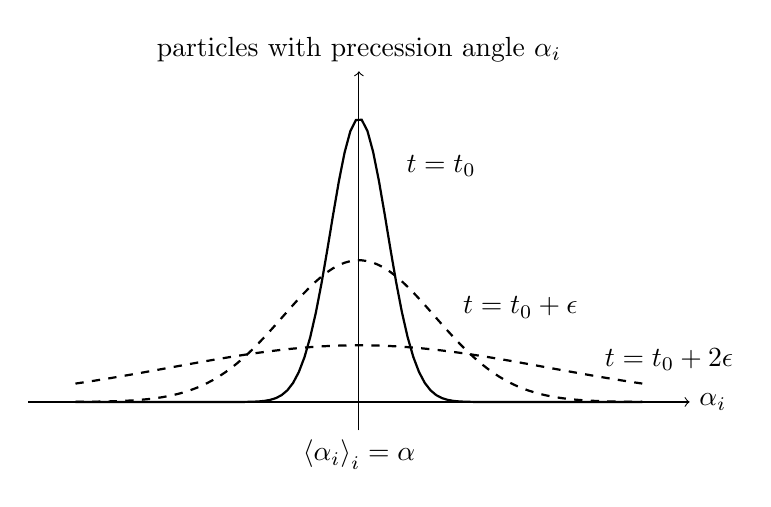
\begin{tikzpicture}[scale=1.2]
    \draw[->] (-3.5,0) -- (3.5,0) node[right] {$\alpha_i$};
    \draw[->] (0,-0.3) -- (0,3.5) node[above] {particles with
    precession angle $\alpha_i$};

    \node[below] at (0,-0.3) {$\left< \alpha_i \right>_i = \alpha$};

    \pgfmathsetmacro{\Anarrow}{3.0}
    \pgfmathsetmacro{\signarrow}{0.3}
    \draw[solid, thick] plot[domain=-3:3, samples=100]
    (\x, {\Anarrow*exp(-(\x)^2/(2*\signarrow^2))});
    \node[right] at (0.4, 2.5) {$t = t_0$};

    \pgfmathsetmacro{\Amedium}{1.5}
    \pgfmathsetmacro{\sigmedium}{0.8}
    \draw[dashed, thick] plot[domain=-3:3, samples=100]
    (\x, {\Amedium*exp(-(\x)^2/(2*\sigmedium^2))});
    \node[right] at (1.0, 1.0) {$t = t_0 + \epsilon$};

    \pgfmathsetmacro{\Awide}{0.6}
    \pgfmathsetmacro{\sigwide}{2.0}
    \draw[dashed, thick] plot[domain=-3:3, samples=100]
    (\x, {\Awide*exp(-(\x)^2/(2*\sigwide^2))});
    \node[right] at (2.5, 0.45) {$t = t_0 + 2\epsilon$};
  \end{tikzpicture}
  \caption{Relaxation due to spin-spin interactions can be
    conceptualized as a distribution with initially low variance centered around
    the average angle of precession of the nuclei that increases in
    variance with time. This distribution loses its center and approaches
    the initial uniform distribution associated with $\vec M$ aligned
    with $\vec B_0$ as discrete time-steps of size $\epsilon$ progress
  toward infinity.}
  \label{fig:gaussian_dispersion}
\end{figure}